\chapter{Development Methodologies}
\label{chapter:development_methodologies}
This chapter discuses the development practices that are used during the development process of the proposed system.  

\section{Development Model}
\label{section:development-model}
As with every software product, specific rules are needed to ensure that the software is developed in a manner that satisfies its specifications and achieves the end-goals. In the IT industry that is achieved by following a software development model. It specifies the required stages of the development and the order in which they are carried out. In this project the \textit{Incremental Model} has been chosen to drive the development of the software. The main idea behind this model is developing a system through iterative steps and in small incremental portions \citep[264]{bhuvaneswari2013}. It ensures that each iteration (e.g. software build) is tested and working before using the previous iteration as a base for the next one (see figure \ref{fig:incremental-model}). The main benefits of using this model are:

\begin{itemize}
    \item A product is produced early in the project's development
    \item Because of the previous point, unforeseen problems can be detected early
    \item Client change requests can be implemented between increments
\end{itemize}

    \begin{figure}[H]
        \centering
        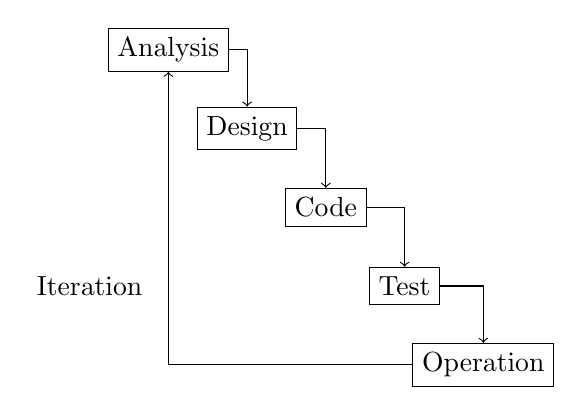
\begin{tikzpicture}
            % nodes
            \node (a1) [draw]  {Analysis};
            \node (d1) [draw, below of=a1, right of=a1] {Design};
            \node (c1) [draw, below of=d1, right of=d1] {Code};
            \node (t1) [draw, below of=c1, right of=c1] {Test};
            \node (o1) [draw, below of=t1, right of=t1] {Operation};
            \node at (-1,-3) {Iteration};
            % arrows
            \draw[->, to path={-| (\tikztotarget)}](a1) edge (d1) (d1) edge (c1) (c1) edge (t1) (t1) edge (o1) (o1) edge (a1);
        \end{tikzpicture}
        \caption{Incremental software development model life cycle}
        \label{fig:incremental-model}
    \end{figure}


\section{Version Control System}
When developing software challenges can occur unexpectedly, and a developer has to do whatever possible to ensure their work is protected. For example, an untraceable bug can be introduced in one of the iterations of the iterative development model (see section \ref{section:development-model}) that could lead to poor system performance. In order to prevent the (or at least dramatically lower)the occurrence these situations, the use of \textit{"Version Control"} is encouraged.

There are many Version Control Systems (VCS) out there such as Mercurial, Fossil and Git. The main purpose of a \gls{vcs} is to keep track of the changes in a project. If a developer is satisfied with a specific change, they can perform a \textit{commit}. That action will merge the change to the codebase, and the commit command will be added to the changelog (list of commits). If there is a problem that has been caused by a previous \textit{"bad"} commit, the developer can simply revert the whole project to a more stable state by restoring the codebase to a previous known \textit{"good"} commit.

For this project, Git has been chosen along with its web service GitHub\footnote{\url{https://github.com}} to serve as a \gls{vcs} due to the fact that it is easy to use and it is well-documented.


\section{Project Management}
It is important to stay organised when it comes to working on a project, especially when it involves the usage of limited resources (i.e. Time). Thus, a project management tool called \textit{Taiga.io}\footnote{\url{https://taiga.io}} was utilised to help keep track of the project's progress via \textbf{\textit{Kanban} boards}. With every incremental iteration (see \ref{fig:incremental-model} above) new tasks are identified, created and added to the Kanban boards.

Using \textit{Kanban} boards introduces several benefits to the development of the project. Firstly, it provides a quick way to organise the project work visually. For example, boards titled \textit{"READY"} and \textit{"IN PROGRESS"} tables contain that tasks that are already implemented and what those that are being implemented, respectively (see figure \ref{fig:taiga-kanban-boards}). Secondly, it increases the development efficiency since one of the key aspects of the Kanban methodology is to limit the work in progress (WIP) by setting a limit \citep[]{atlassian2017}. For example, if the number of tasks in \textit{IN-PROGRESS} board is 1, that means that no other tasks should be started until the currently undergoing one is finished.

\begin{figure}[ht]
    \centering
    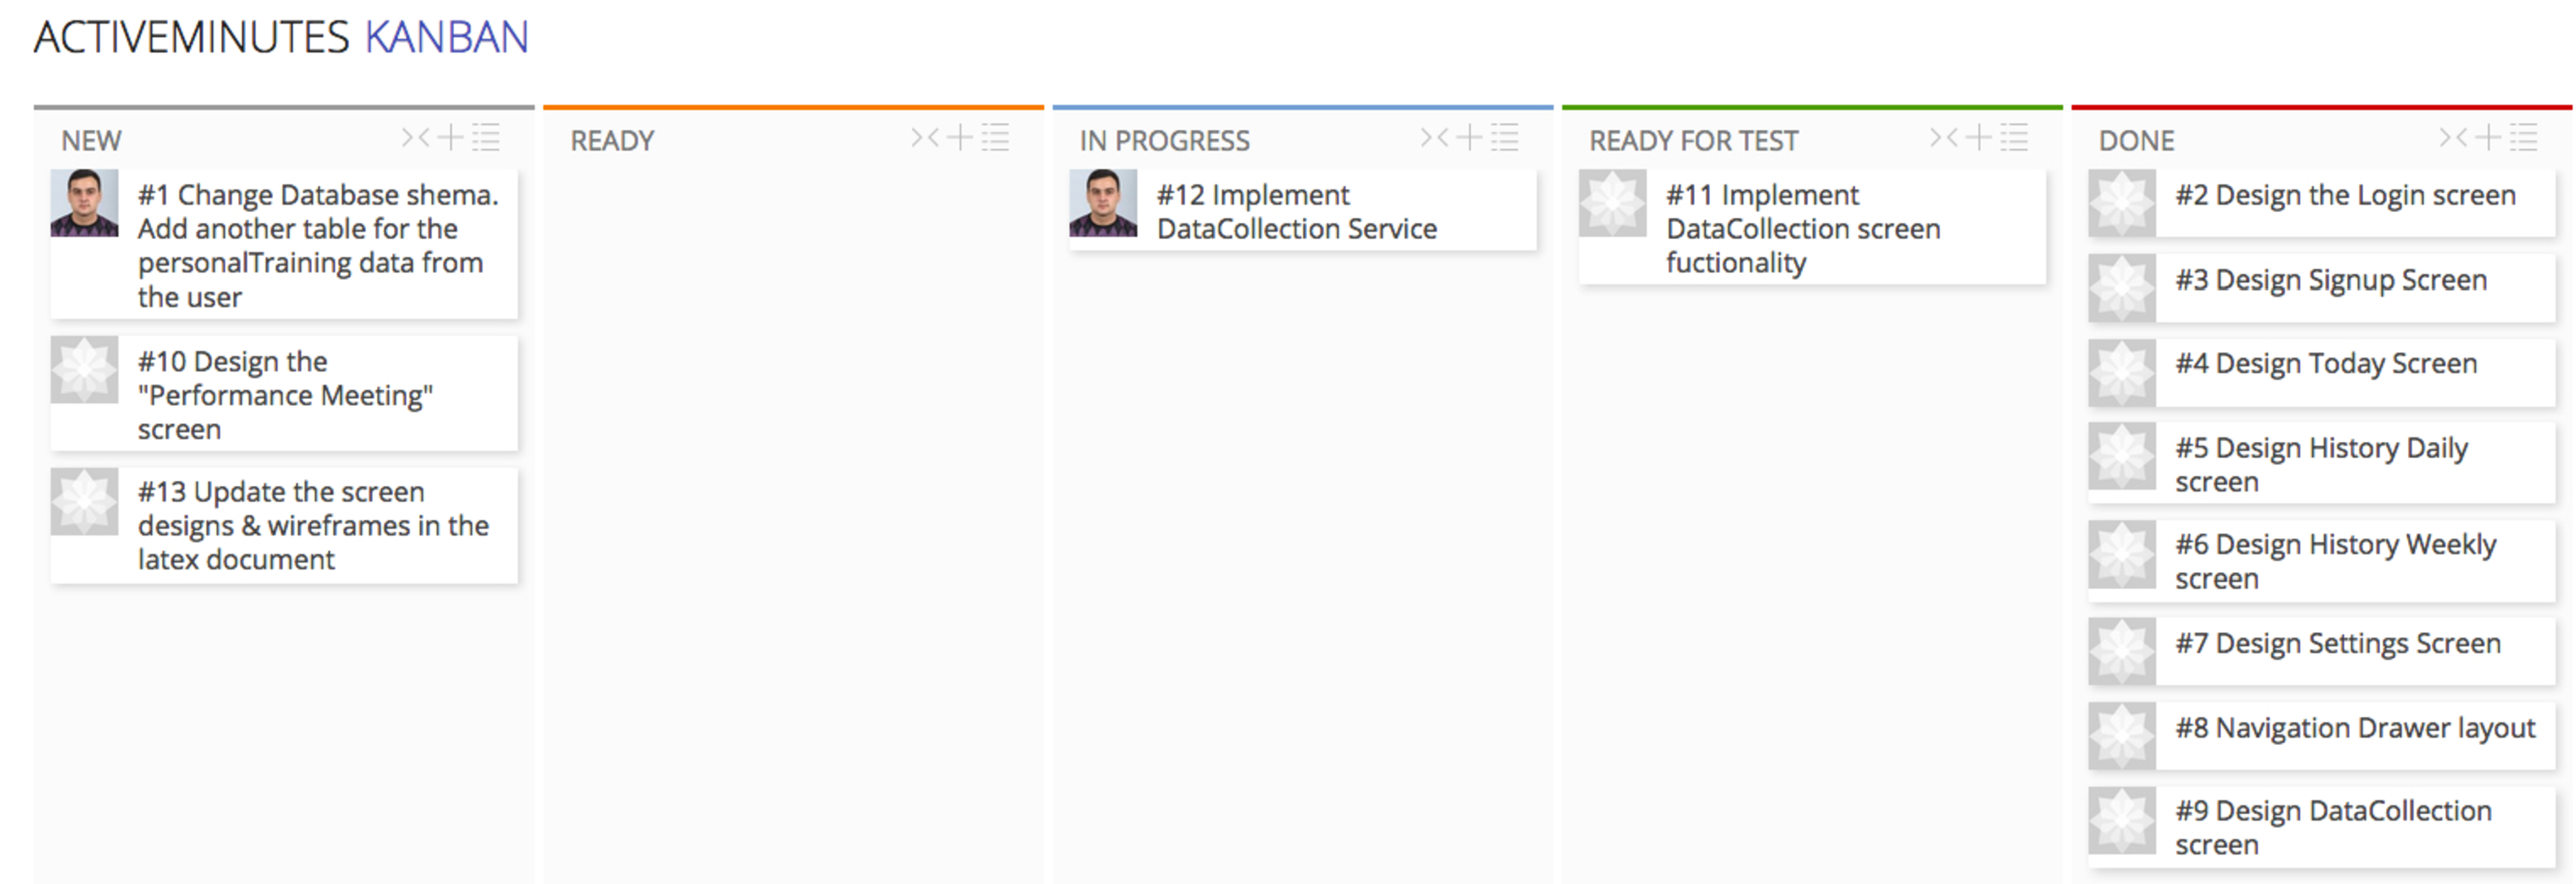
\includegraphics[width=15cm]{taiga-kanban-boards}
    \caption{Taiga Kanban boards}
    \label{fig:taiga-kanban-boards}
\end{figure}

\section{MVP and Dependency Injection}
    As discussed before, the implementation of the mobile application is following the \gls{mvp} software pattern, which allows for the clear separation of code concepts (see section \ref{section:architectural-design}). To better satisfy the requirements discussed in section \ref{section:system-quality-attributes}, \gls{mvp} is combined with a Dependency Injection (DI) principle. What \gls{di} do is shifting the responsibility of one class to create its dependencies to another class. For example, class Car requires class Engine as a parameter. Instead of creating a new instance of class Engine when class Car is created it is simply provided as a constructor parameter in class Car's constructor (see listing \ref{di-car-example}).
    
     \begin{wrapfigure}{RI}{0.3\textwidth}
        \begin{center}
            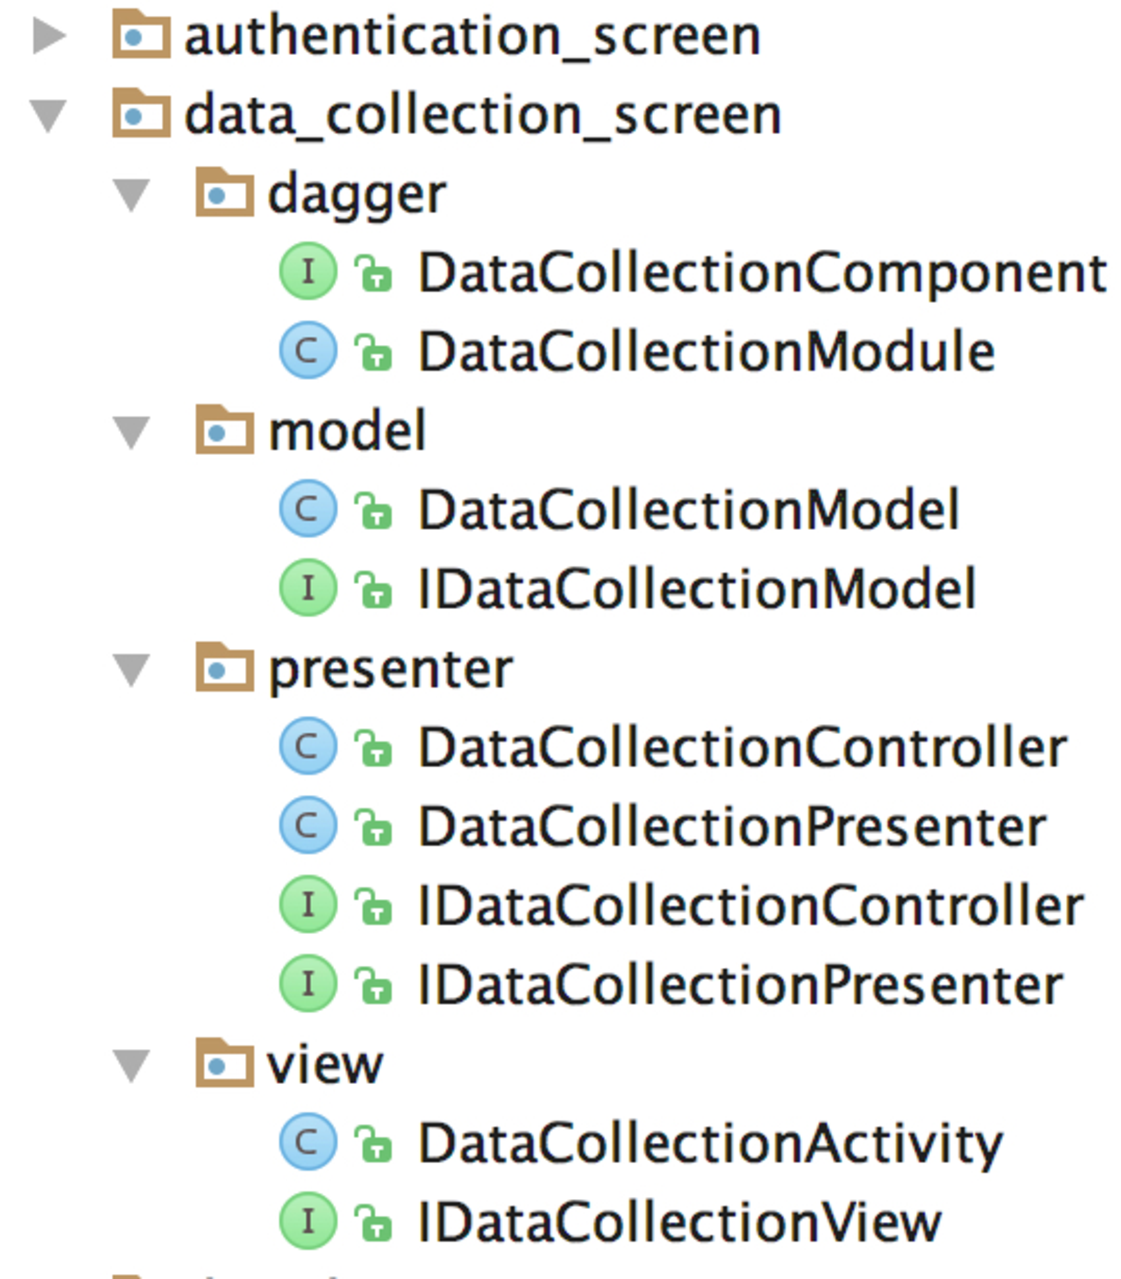
\includegraphics[width=0.3\textwidth]{app-directory-structure}
        \end{center}
    \caption{Data collection screen directory structure}
    \label{fig:app-directory-structure}
    \end{wrapfigure}
    
    Dagger\footnote{\url{https://github.com/google/dagger}} is a framework that utilises the \gls{di} principle in the form of \textit{Component} and \textit{Module} classes. A module creates the necessary dependencies (e.g. object of class B) whereas the Component class determines where those dependencies will be "injected" (e.g. satisfy dependence's in class A). A concrete example of \gls{di} can be seen in Listing \ref{di-example}. In this example, the \textbf{LoginFragment} (e.g. the login screen) requires an object of type \textit{\textbf{"ILoginPresenter"}} to function. The method \textit{\textbf{"satisfyDependencies()"}} provides the dependencies to the class (e.g. externally). All of the dependencies of the Login screen are provided from a Dagger module named \textit{\textbf{"AuthModule"}} which is responsible for providing and creating the concrete implementation of the above interface (e.g. ILoginPresenter). The full code of \textit{\textbf{"AuthModule"}} as well as \textit{\textbf{"AuthComponent"}} can be seen in Appendix \ref{chapter:dagger-component-module}.  
    
        
    Combining the \gls{mvp} design pattern with dependency injection framework such as Dagger brings many advantages for the software product. Firstly, the software becomes more loosely coupled as the \gls{mvp} enforces the use of interfaces and Dagger is responsible for injecting the concrete implementation of those interfaces where required. Secondly, it allows for logically structuring the codebase. For example, a common approach when using both \gls{mvp} and Dagger is to create a directory for each one of the mobile screens (see figure \ref{fig:app-directory-structure}) containing the necessary \gls{mvp} classes such as \textit{\textbf{Presenter}} and \textit{\textbf{Model}} and the as well as Dagger's \textit{\textbf{Module}} and \textit{\textbf{Component}} to handle the \gls{di} process.
    
\begin{lstlisting}[caption= DI example, label=di-car-example,frame=tlrbr,basicstyle=\small,captionpos=b]
    class Car{
        Engine engine;
            Car(Engine engine){
                this.engine = engine;
            }
       }
    }
\end{lstlisting}
